% ******************************************************** %
%              TEMPLATE DE INFORME ORGA2 v0.1              %
% ******************************************************** %
% ******************************************************** %
%                                                          %
% ALGUNOS PAQUETES REQUERIDOS (EN UBUNTU):                 %
% ========================================
%                                                          %
% texlive-latex-base                                       %
% texlive-latex-recommended                                %
% texlive-fonts-recommended                                %
% texlive-latex-extra?                                     %
% texlive-lang-spanish (en ubuntu 13.10)                   %
% ******************************************************** %


\documentclass[a4paper]{article}
\usepackage[spanish]{babel}
\usepackage[utf8]{inputenc}
\usepackage{charter}   % tipografia
\usepackage{graphicx}
%\usepackage{makeidx}
\usepackage{paralist} %itemize inline

%\usepackage{float}
%\usepackage{amsmath, amsthm, amssymb}
%\usepackage{amsfonts}
%\usepackage{sectsty}
%\usepackage{charter}
%\usepackage{wrapfig}
%\usepackage{listings}
%\lstset{language=C}
\usepackage{caption}

% \setcounter{secnumdepth}{2}
\usepackage{underscore}
\usepackage{caratula}
\usepackage{url}
\usepackage[document]{ragged2e}
\usepackage[export]{adjustbox}
\usepackage{subcaption}
\usepackage{floatrow}


% ********************************************************* %
% ~~~~~~~~              Code snippets             ~~~~~~~~~ %
% ********************************************************* %

\usepackage{color} % para snipets de codigo coloreados
\usepackage{fancybox}  % para el sbox de los snipets de codigo

\definecolor{litegrey}{gray}{0.94}

\newenvironment{codesnippet}{%
	\begin{Sbox}\begin{minipage}{\textwidth}\sffamily\small}%
	{\end{minipage}\end{Sbox}%
		\begin{center}%
		\vspace{-0.4cm}\colorbox{litegrey}{\TheSbox}\end{center}\vspace{0.3cm}}



% ********************************************************* %
% ~~~~~~~~         Formato de las páginas         ~~~~~~~~~ %
% ********************************************************* %

\usepackage{fancyhdr}
\usepackage{parskip}
\pagestyle{fancy}

%\renewcommand{\chaptermark}[1]{\markboth{#1}{}}
\renewcommand{\sectionmark}[1]{\markright{\thesection\ - #1}}

\fancyhf{}

\fancyhead[LO]{Sección \rightmark} % \thesection\
\fancyfoot[LO]{\small{Luis Enrique Badell Porto, Nicolas Bukovits, Kevin Frachtenberg}}
\fancyfoot[RO]{\thepage}
\renewcommand{\headrulewidth}{0.5pt}
\renewcommand{\footrulewidth}{0.5pt}
\setlength{\hoffset}{-0.8in}
\setlength{\textwidth}{16cm}
%\setlength{\hoffset}{-1.1cm}
%\setlength{\textwidth}{16cm}
\setlength{\headsep}{0.5cm}
\setlength{\textheight}{25cm}
\setlength{\voffset}{-0.7in}
\setlength{\headwidth}{\textwidth}
\setlength{\headheight}{13.1pt}
\setlength{\parindent}{4em}
\setlength{\parskip}{\baselineskip}

\renewcommand{\baselinestretch}{1.1}  % line spacing

% ******************************************************** %


\begin{document}


\thispagestyle{empty}
\materia{Organización del Computador II}
\submateria{Primer Cuatrimestre de 2016}
\titulo{Trabajo Práctico 2}
\subtitulo{Procesamiento de imágenes con SIMD}
\integrante{Luis Enrique Badell Porto}{246/13}{luisbadell@gmail.com}
\integrante{Nicolas Bukovits}{546/14}{nicko_buk@hotmail.com}
\integrante{Kevin Frachtenberg}{247/14}{kevinfra94@gmail.com}
\grupo{Grupo: Yo no manejo el raiting, yo manejo un Rolls-Royce}
\maketitle

%{\small\textbf{\flushleft{Resumen}}\\
\abstract {En el siguiente trabajo pr\'actico, se busca analizar, estudiar y comprender el funcionamiento y rendimiento de la tecnolog\'ia
SIMD (Single Instruction Multiple Data) inclu\'ida en el sistema SSE de los procesadores Intel. Para esto, se realizaron tres filtros
de im\'agenes (Cropflip, Sepia y Low Dynamic Range) en lenguaje C y en lenguaje ensamblador para aplicar sobre imagenes BMP, y luego se comparó el rendimiento entre ellos.
Los resultados obtenidos de estos experimentos, fueron plasmados y analizados en este informe.
}

%\newpage

%\thispagestyle{empty}
%\vfill


\thispagestyle{empty}
\vspace{3cm}
\tableofcontents
\newpage


%\normalsize
\newpage



\section{Introduccion}
\subsection{Cropflip}
El filtro cropflip recibe como parametros extra dos tamaños y dos offset. Un tamaño y un offset para las filas, y los otros dos para las columnas.
Lo que se hace con esto es recortar la imagen original en una nueva imagen e invertirla verticalmente. La imagen se recorta desde
donde los offsets lo indican hasta el tamaño indicado.
\newline
Ejemplo: cropflip lena32.bmp 128 128 40 50

\begin{figure}[!ht]
    \centering
    \begin{floatrow}
      \ffigbox[\FBwidth]{\caption{Antes del filtro cropflip (escala 25\%)}}{%
        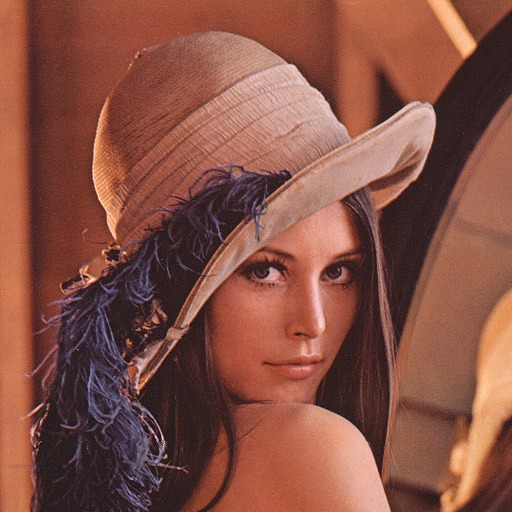
\includegraphics[scale=.25]{./imagenes/lena32.jpg}
      }
      \ffigbox[\FBwidth]{\caption{Después del filtro cropflip (escala 50\%)}}{%
       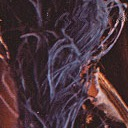
\includegraphics[scale=.50]{./imagenes/lena32-cropflip.jpg}
      }
    \end{floatrow}
\end{figure}

Para el caso de la implementación en lenguaje C, el código toma pixel por pixel y lo copia al lugar correspondiente (invirtiendo la imagen)
en la imagen destino.
Por otro lado, el caso de la implementación en lenguaje ensamblador, utilizamos los registros XMM para que el código lea y copie de a 4 pixels
en la imagen final.

\subsection{Sepia}
El filtro sepia, es el conocido filtro de imagenes que simula una foto antigüa. Para lograr este efecto, lo que se hace es una suma
de los canales de color (R, G, B. Llamaremos a esta suma ``SumaRGB'') y luego se multiplica por un valor fijo para cada canal (0.5 para el canal R, 0.3 para el G
y 0.2 para el canal B). Luego, manteniendo la transparencia en caso de haber, el pixel quedaría conformado por A = A, R = SumaRGB*0.5
, G = SumaRGB*0.3 y B = SumaRGB*0.2. \newline
Al igual que en Cropflip, en el caso de C se trabaja pixel por pixel, mientras que en el caso del lenguaje ensamblador se trabaja un poco diferente:
Si bien se lee de a 4 pixeles de la imagen original, luego es necesario trabajar pixel por pixel ya que cada canal tiene un tamaño de 1 byte
y si quisiéramos realizar la suma de los 3 canales de los 4 pixeles en un solo registro, ésta no entraría en un byte. Así, lo que se hace
es expandir (unpack) cada pixel para que cada canal pase a tener un tamaño de word (2 bytes). Así, la suma máxima será de 255 + 255 + 255, y esto sí
entra en un espacio de tamaño word. Sin embargo, las instrucciones que provee el procesador Intel para multiplicar por floats, nos obliga
a realizar otra expanción (unpack) de cada pixel, pero esta vez de word a Double word (4 bytes, mismo tamaño que un float).
Una vez están listos los cálculos de cada uno de los 4 pixels, se realizan 2 packs para llevar cada canal de doubleword a byte nuevamente.
\newline
Ejemplo: sepia foto.bmp
\begin{figure}[!ht]
    \centering
    \begin{floatrow}
      \ffigbox[\FBwidth]{\caption{Antes del filtro sepia}}{%
        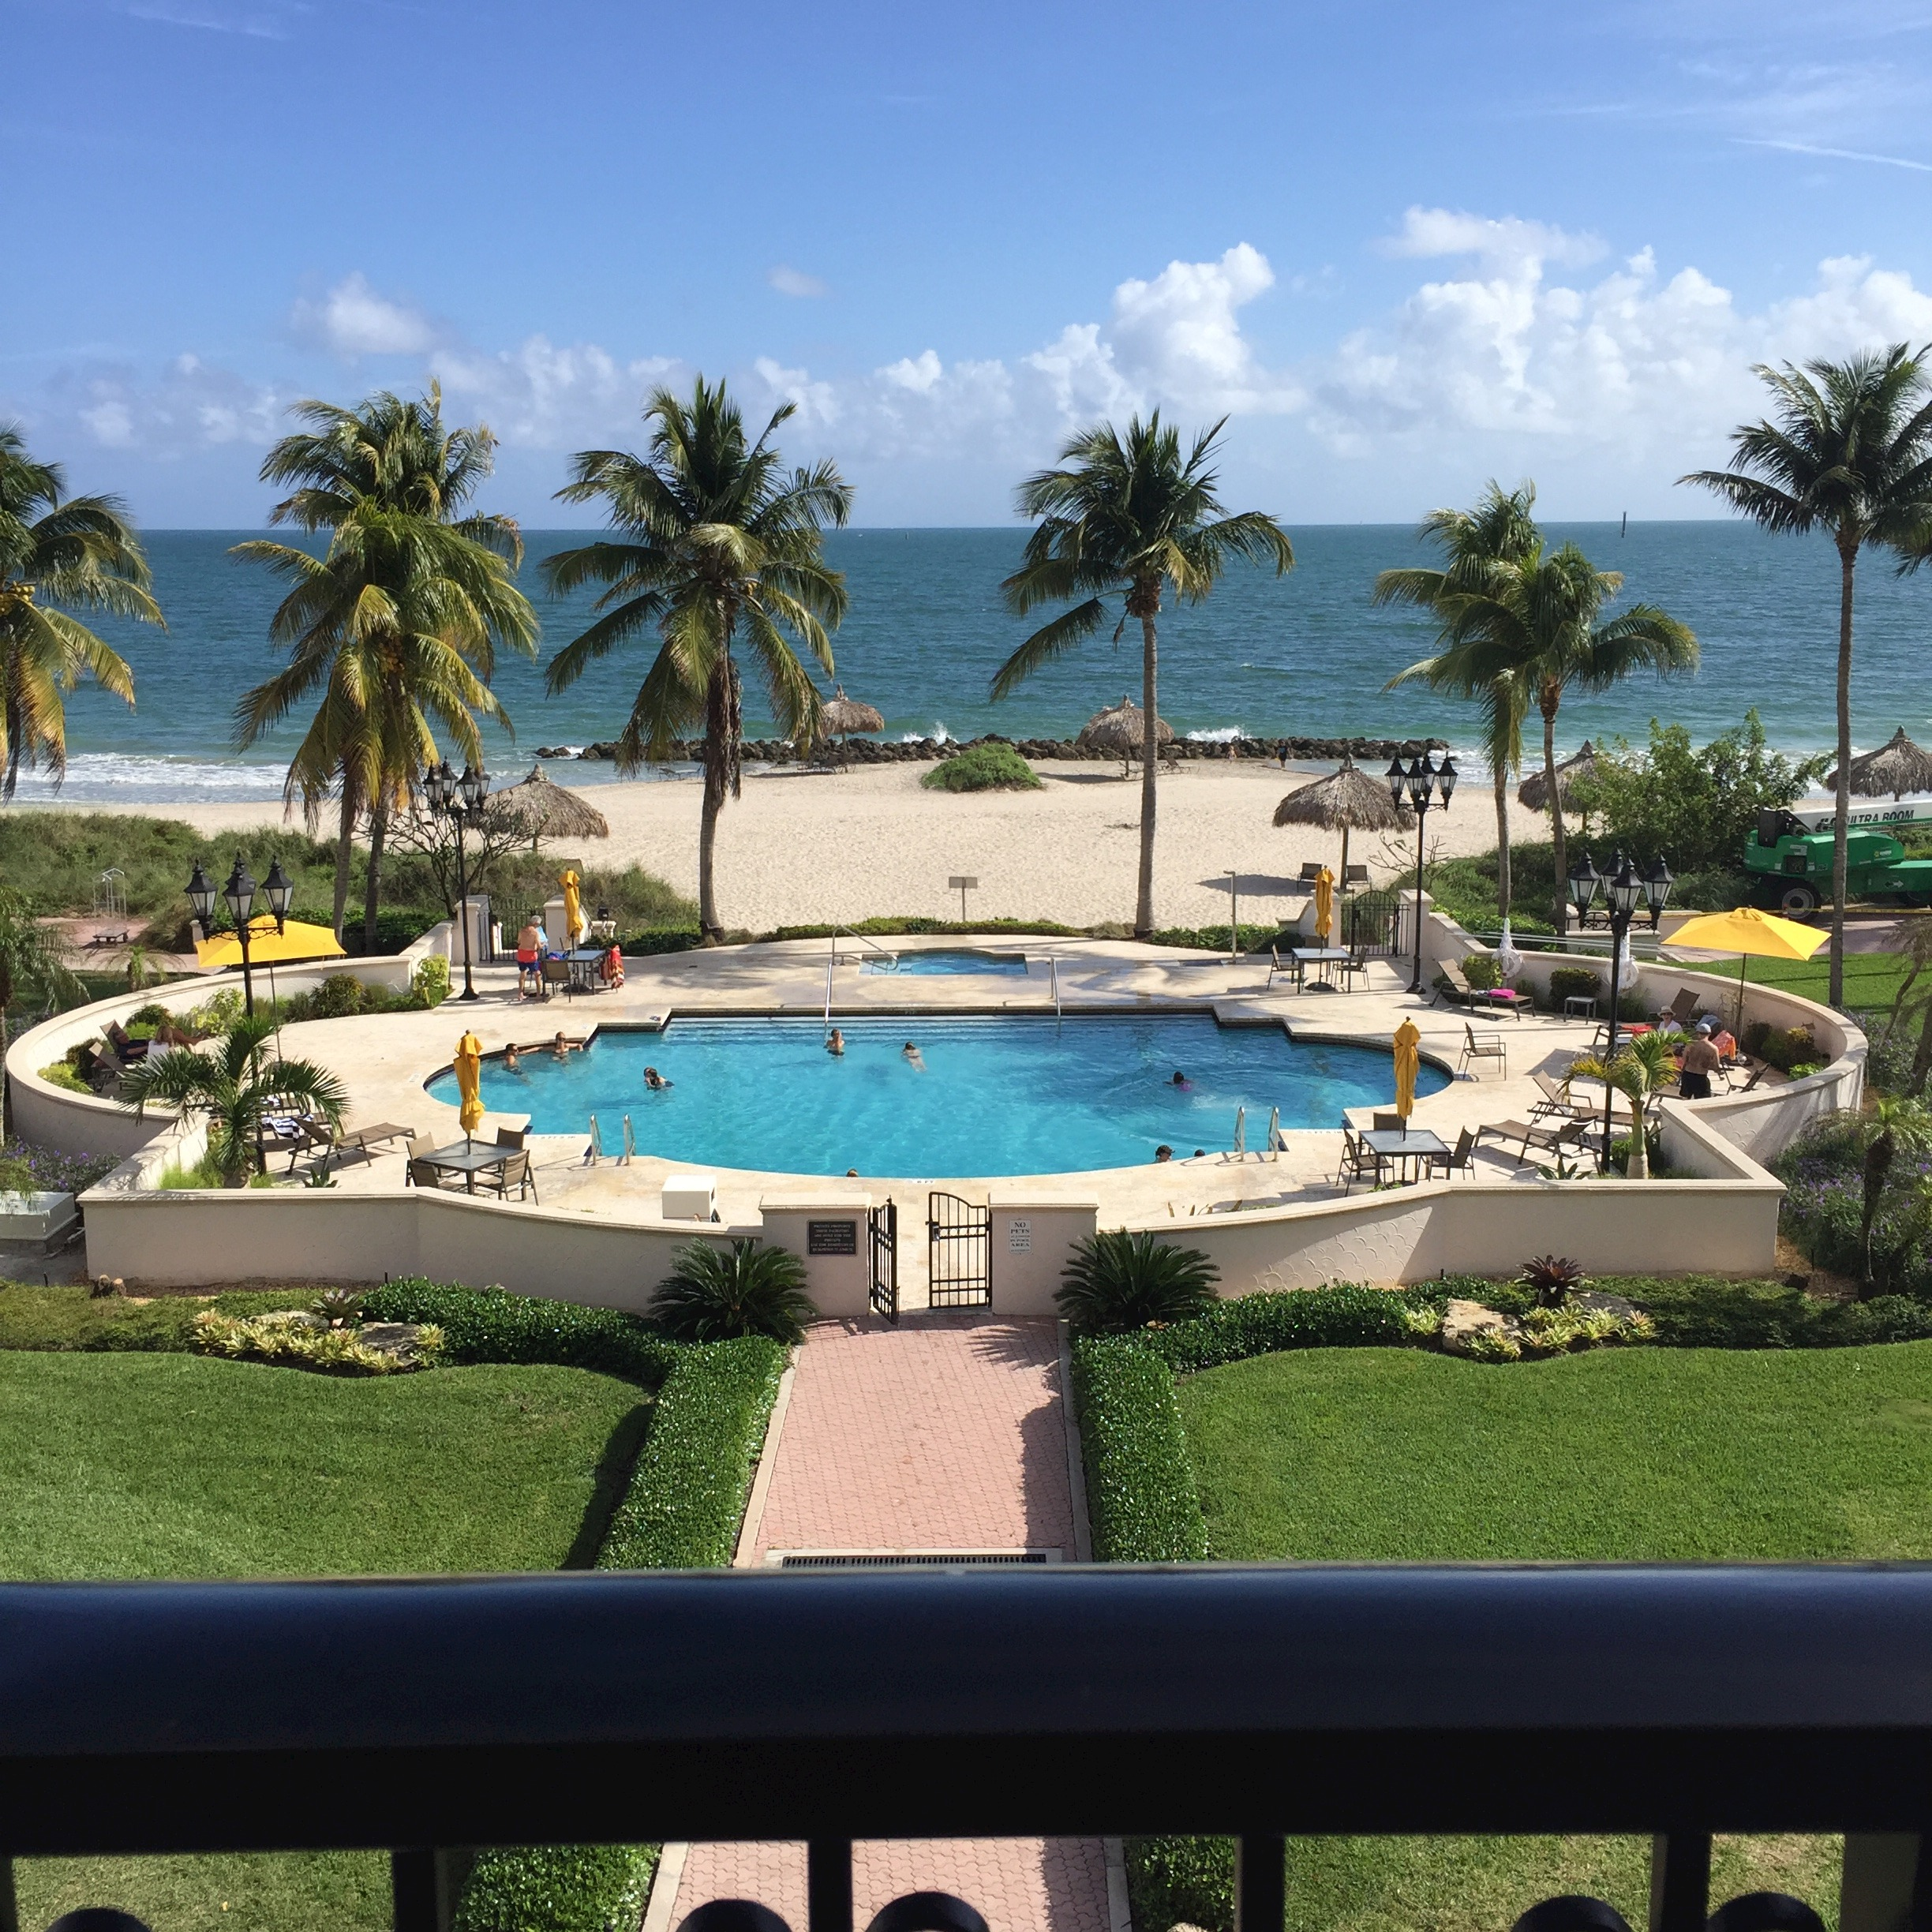
\includegraphics[scale=.04]{./imagenes/foto.jpg}
      }
      \ffigbox[\FBwidth]{\caption{Después del filtro sepia}}{%
       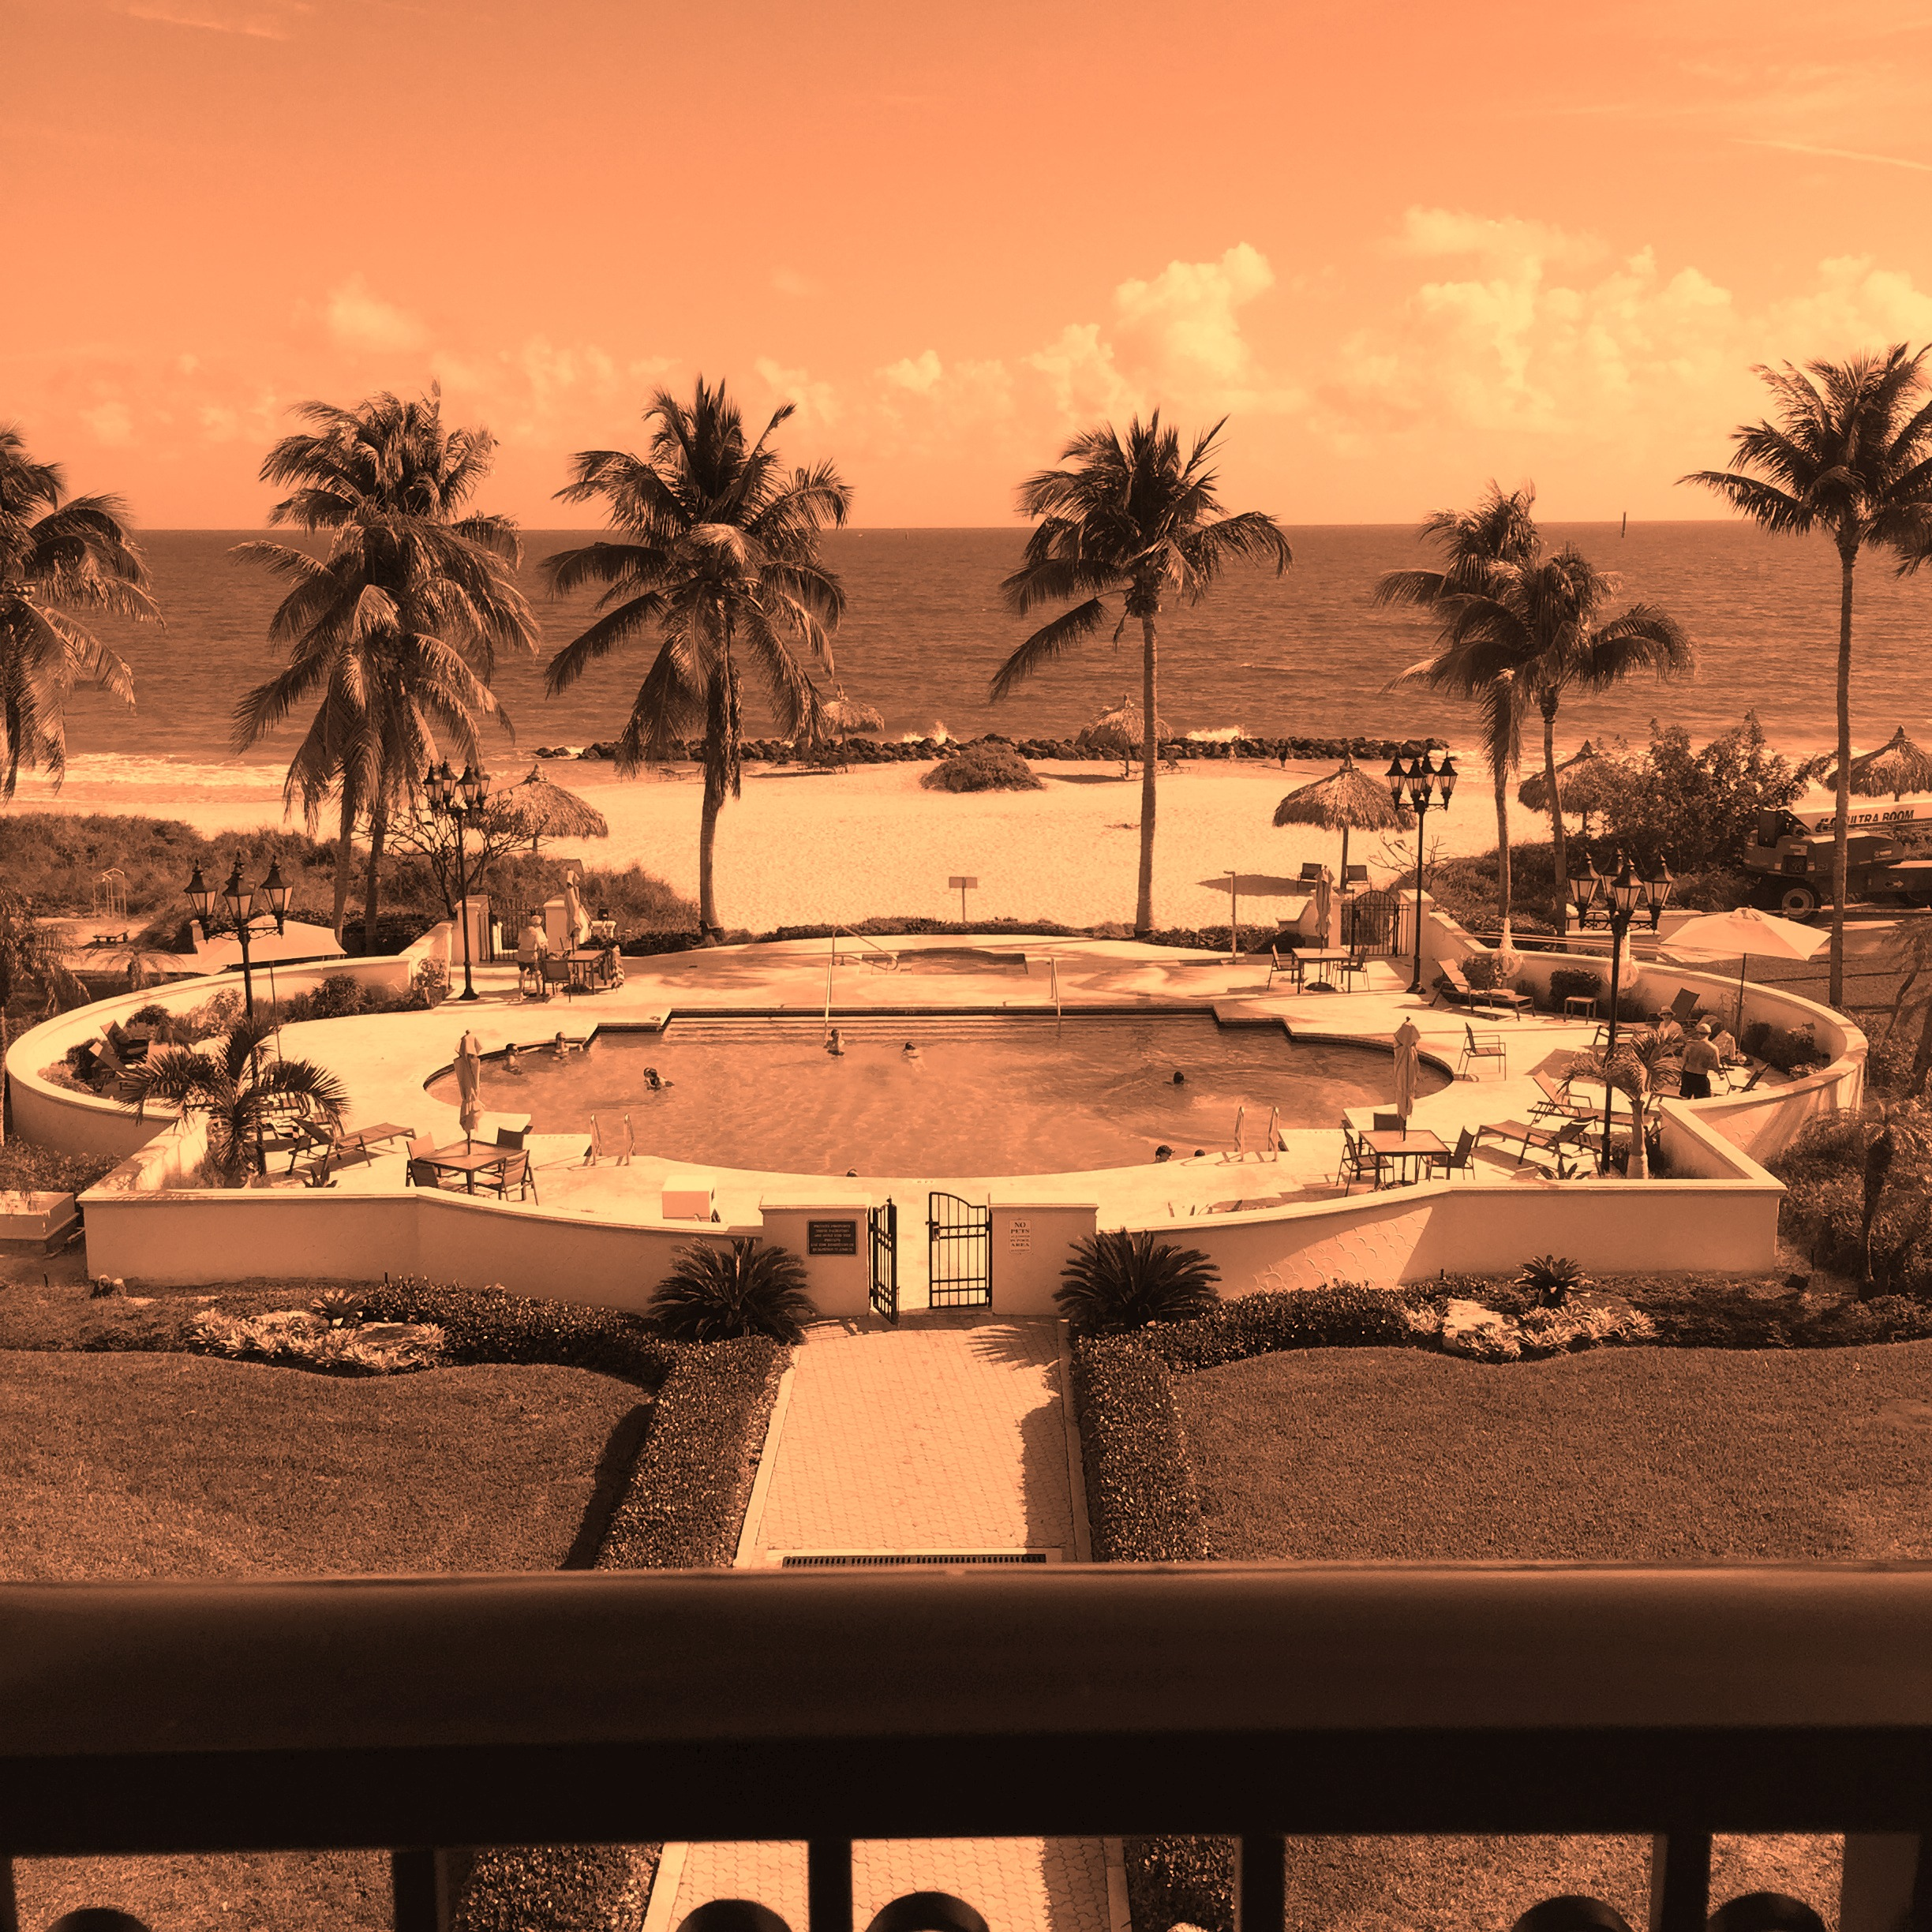
\includegraphics[scale=.04]{./imagenes/foto-sepia.jpg}
      }
    \end{floatrow}
\end{figure}

\subsection{Low Dynamic Range}
Este filtro, más conocido como LDR, se logra realizando una serie de cálculos en base a los 25-vecinos de cada pixel del interior
de la imagen (si tomamos ``interior'' como 2 pixels hacia adentro desde cada borde), y a un $\alpha$ pasado por parámetro, el cual puede ser
un valor entre -255 y 255. Lo que hace el filtro es agregar o quitar luminosidad dependiendo del $\alpha$. El método para lograr este efecto es
modificar cada canal de color (R,G,B) del pixel a revisar, a través de realizar una suma de los 3 canales de color de los 25-vecinos del pixel a editar (incluyendo el mismo pixel),
luego se multiplica ese valor por el $\alpha$ y por el valor del canal del pixel en observación. Por último, se divide por un valor ``Max'',
que se da haciendo el cálculo del posible máximo del cálculo anterior (255*25*3*255); se suma el valor del canal antes multiplicado y antes
de guardarse, se satura a 0 o 255, que es el maximo de cada canal (ya que como el $\alpha$ puede ser negativo, es necesario tomar el caso
en que quede un número negativo en el canal).
\newline
El caso de C es igual a sepia y cropflip: Se analiza pixel por pixel. El caso del lenguaje ensamblador es parecido, ya que no se pueden
hacer cálculos tan grandes con 4 pixeles al mismo tiempo. Es por esto, que también se analiza pixel por pixel, pero para realizar el
cálculo de la suma de los 25 vecinos, las multiplicaciones, la división, suma y saturación, se utilizan instrucciones SSE.
\newline
Ejemplo: ldr bob.bmp 100
\begin{figure}[!ht]
    \centering
    \begin{floatrow}
      \ffigbox[\FBwidth]{\caption{Antes del filtro ldr}}{%
        
\includegraphics[scale=.25]{./imagenes/bob.jpg}
      }
      \ffigbox[\FBwidth]{\caption{Después del filtro ldr}}{%
       
\includegraphics[scale=.25]{./imagenes/bob-ldr.jpg}
      }
    \end{floatrow}
\end{figure}


\section{Desarrollo}

\subsection{Hipótesis y bases}
Nosotros tenemos como hipótesis que dadas las herramientas que nos ofrece la tecnología SSE, y que nosotros mismos somos los que nos
ocupamos de hacer una buena implementación en cada lenguaje, los algoritmos hechos en lenjuage ensamblador serán mucho más rápidos
que los que están hechos en lenguaje C. Sabemos que parte del retraso que tiene el lenguaje C se debe a que es el compilador quien decidirá cómo
optimizar el algoritmo implementado; esto es, traducir a código de máquina según la interpretación que le de el compilador al código C. Es por esto
que usaremos el flag O3 como caso de compilación extra, y así poder comparar distintos métodos de compilación sobre una misma
implementación del lenguaje C.
Para el caso del lenjuage ensamblador, no hay un compilador de por medio, ya que es simplemente traducir a código de máquina desde las instrucciones
escritas.
\newline
Para poder comparar cada implementación de los filtros, los mismos se ejecután reiteradas veces en imagenes de distintos tamaños.
De cada ejecución, tomaremos el tiempo del clock antes de correr el programa y después de correrlo, y así observaremos
la cantidad de ciclos de reloj que toma cada vez. Si bien esto puede traer problemas como por ejemplo el tema de los \textit{outliers},
por razones de probabilidad y estadística, un promedio de cantidades grandes se acercará más a un promedio real.

\subsection{Implementación y Análisis}

\subsubsection{Cropflip}
Como se mencionó en la introducción, el filtro de Cropflip toma, en el caso de C, cada pixel y se copia de memoria a memoria.
Sabemos que en la práctica esto solo funciona con un DMA, por lo que depende del compilador decidir cómo hacer las iteraciones para
recorrer la imagen original y copiar cada pixel a la nueva posición de memoria.
Para el caso de ASM, se toma de a 4 pixels y se mueven a un registro XMM. dado que un pixel tiene tamaño de 32 bits y el tamaño
del registro XMM es de 128, hacer esto es posible mediante instrucciones SSE (en este caso, movdqu). Luego lo mueve nuevamente a memoria
en la posición correspondiente para ese pixel en la nueva imagen.
Para este filtro, los tests que se realizaron consideraron distintos offsets y se realizaron sobre imágenes de distintos tamaños.
\newline
Los parámetros utilizados para esta experimentación fueron tamx: 128, tamy: 128, offsetx: i-128, offsety: i-128. Donde \textit{i} es
el tamaño de un lado de la imagen, que al ser cuadradas y múltiplos de 4, hace que sea indiferente el lado a elegir.
Este Offset permite tener en cuenta el desplazamiento que debe realizarse para empezar a copiar la imagen, el cual es hasta el último
bloque de 128x128 de la imagen original.
\newline
El primer caso de comparación es la implementación en C compilado sin el Flag O3 contra la implementación en ASM. En el siguiente gráfico
se puede observar la diferencia de tiempo de cada implementación en ciclos de reloj en función del tamaño de la imagen en pixels.

% \begin{figure}[!ht]
%     \centering
%     \begin{floatrow}
%       \ffigbox[\FBwidth]{\caption{Comparación C sin optimizar vs ASM}}{%
%         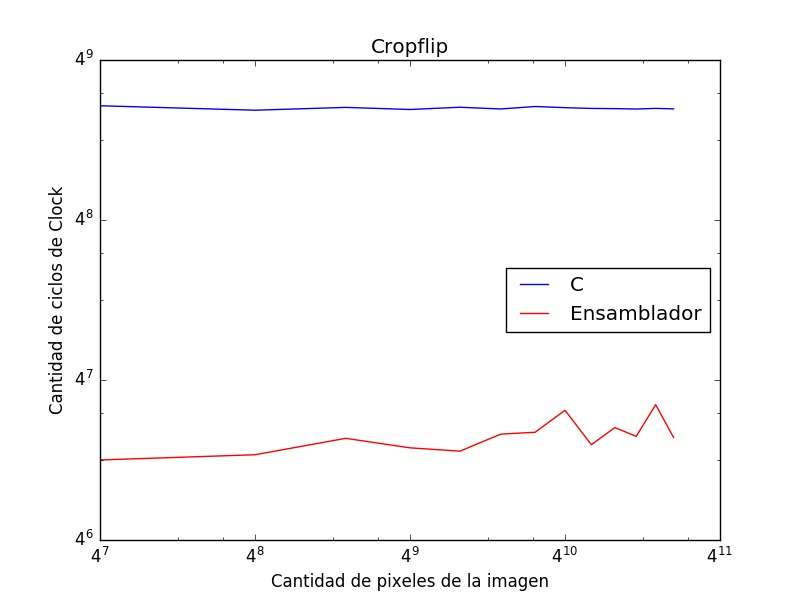
\includegraphics[scale=.55]{./imagenes/Cropflip0.jpeg}%cropflip-asmVSc.jpeg}
%       }
%     \end{floatrow}
% \end{figure}
\begin{centering}
	\ffigbox[\FBwidth]{\caption{Comparación C sin optimizar vs ASM}}{%
		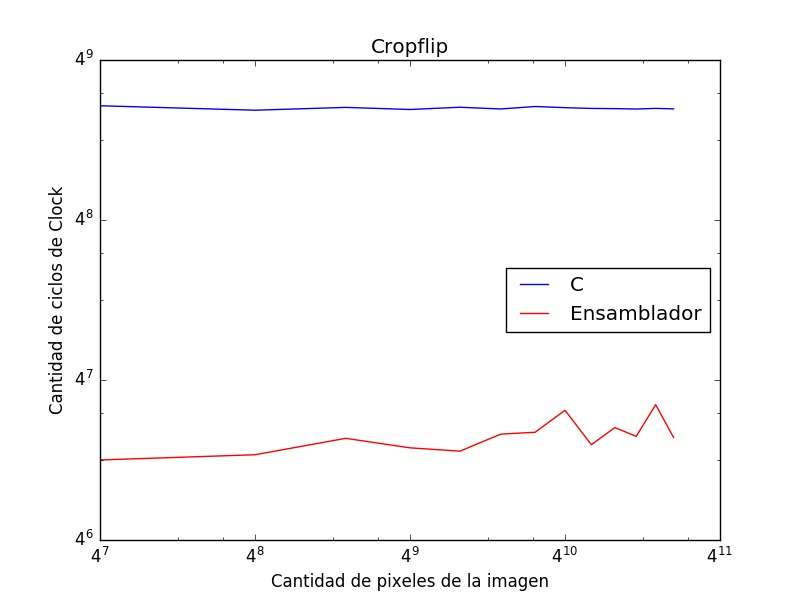
\includegraphics[scale=.55]{./imagenes/Cropflip0.jpeg}
	}
\end{centering}

Observamos en este experimento que si bien la implementación en C está basada en la misma idea que la implementación en ASM,
el código generado por el compilador hace que tome mucho más tiempo resolver cada aplicación del filtro hasta el punto de crecer linealmente
respecto del tamaño de la imágen. Podemos entender esto como una muestra de la diferencia en capacidad de procesamiento de los procesadores que utilizan
la tecnología SSE contra los que no la utilizan o no tienen. Según las muestras tomadas, obtuvimos como resultado que la versión en C es casi 16 veces
más lenta que la versión en ASM.

% \begin{figure}[!ht]
%      \centering
% 		 \begin{floatrow}
% 		 \ffigbox[\FBwidth]{\caption{Comparación C con optimización O3 vs ASM}}{%
%      		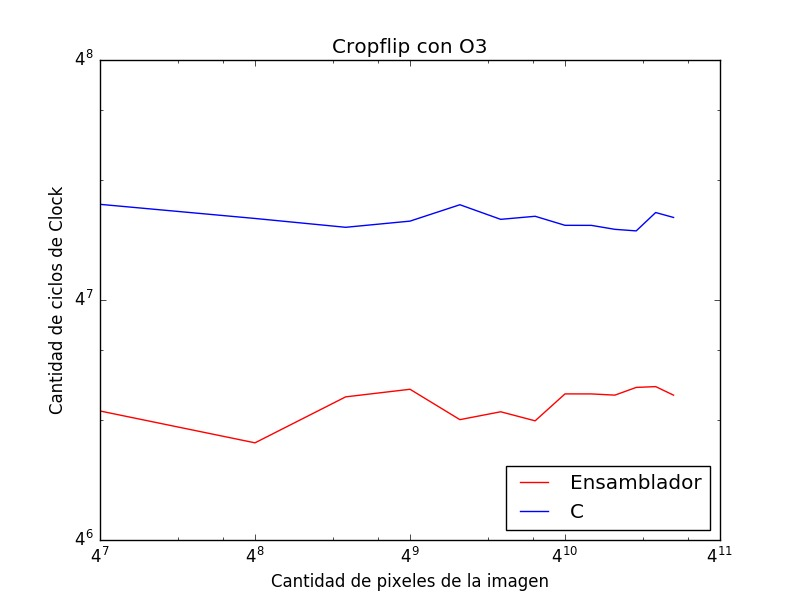
\includegraphics[scale=.55]{./imagenes/Cropflip3.jpeg}%cropflip-asmVScO3.jpeg}
%      }
%    \end{floatrow}
% \end{figure}
\begin{centering}
\ffigbox[\FBwidth]{\caption{Comparación C con optimización O3 vs ASM}}{%
	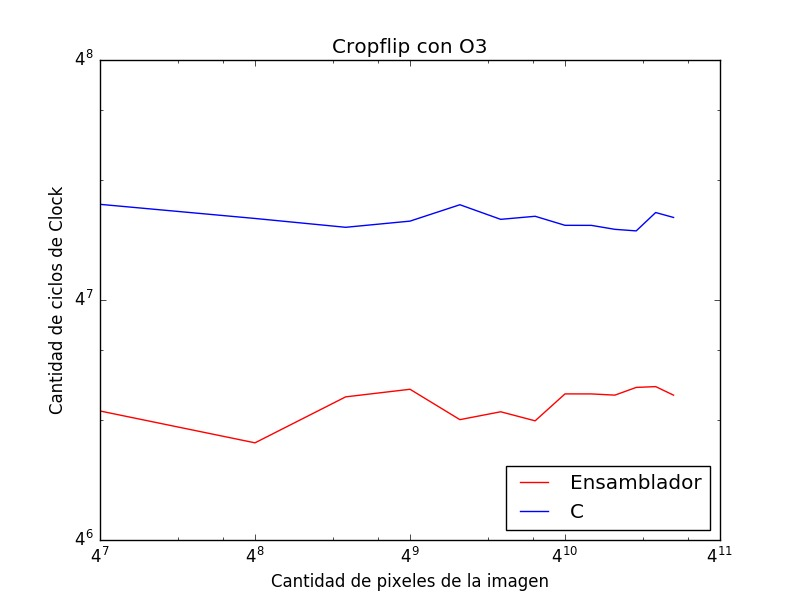
\includegraphics[scale=.55]{./imagenes/Cropflip3.jpeg}
	}
\end{centering}

En este segundo experimento, comparamos la misma implementación C que el caso anterior pero esta vez compilado con el flag O3,
el cual permite compilar el código utilizando tecnología SSE. Si bien se puede observar una amplia mejora (casi 4 veces más rápida) respecto de la versión
sin el flag O3, aún se nota mucha diferencia en comparación con la versión de ASM. Siguiendo las muestras, la versión ASM es aproximadamente 4 veces más rápida
que la versión en C con optimización O3.
\newline

Para el siguiente cuadro comparativo se utilizó también el flag que permite utilizar tecnología AVX, el cual contiene acceso
a registros de 256-bits. A pesar de esto, no hubo una gran mejora de rendimiento respecto de la compilación sin el flag AVX.


\begin{centering}
\ffigbox[\FBwidth]{\caption{Comparación C con optimización O3 y AVX vs ASM}}{%
	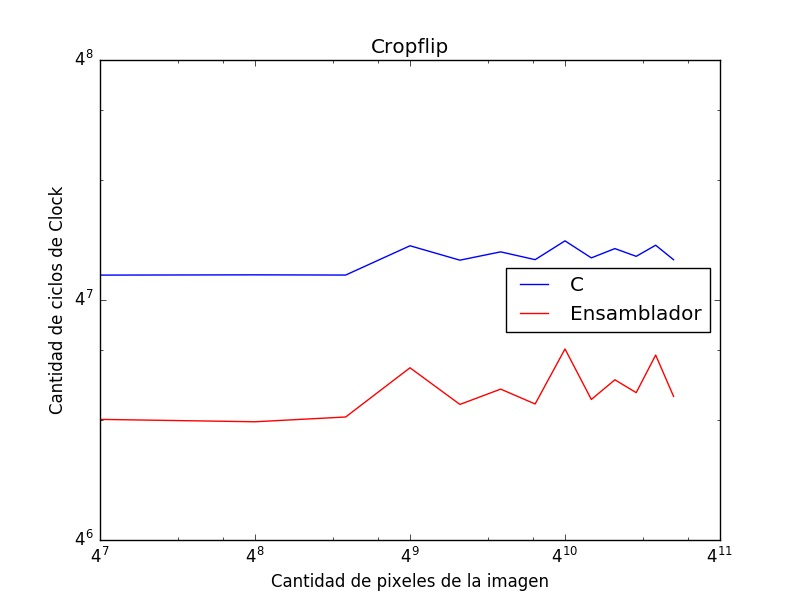
\includegraphics[scale=.55]{./imagenes/cropflip-asmVScO3AVX.jpeg}
	}
\end{centering}

\newpage

\subsubsection{Sepia}
Para el filtro Sepia, al no recibir parámetros extra, se decidió solamente evaluar con distintos tamaños de imágenes.
Esta es la única variable en juego, por lo que se puede analizar mejor cómo varía el filtro entre ASM y C en cuanto a ciclos de clock
respecto del tamaño de la imagen.

%\begin{figure}[!ht]
%    \centering
%    \begin{floatrow}
%      \ffigbox[\FBwidth]{\caption{Comparación C sin optimización vs ASM}}{%
%        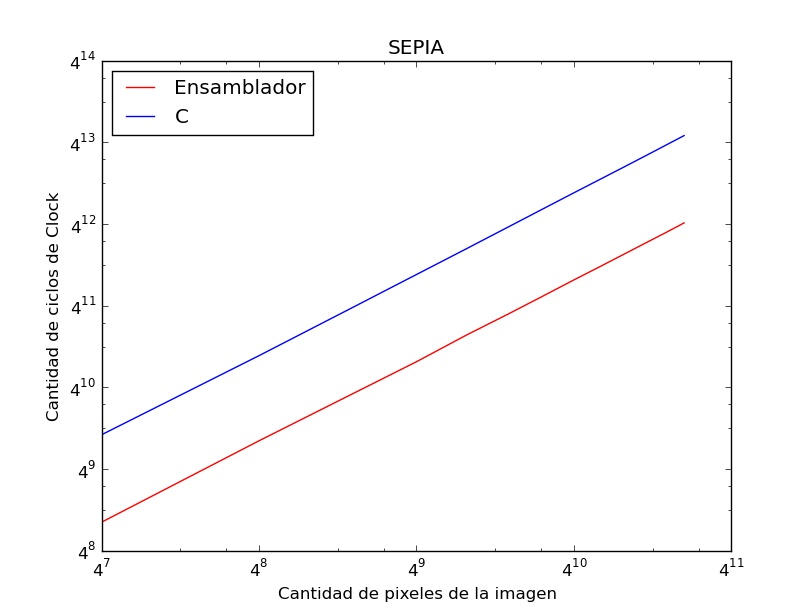
\includegraphics[scale=.25]{./imagenes/sepia-asmVSc.jpeg}
%      }
%    \end{floatrow}
%\end{figure}
\begin{centering}
\ffigbox[\FBwidth]{\caption{Comparación C sin optimización vs ASM}}{%
	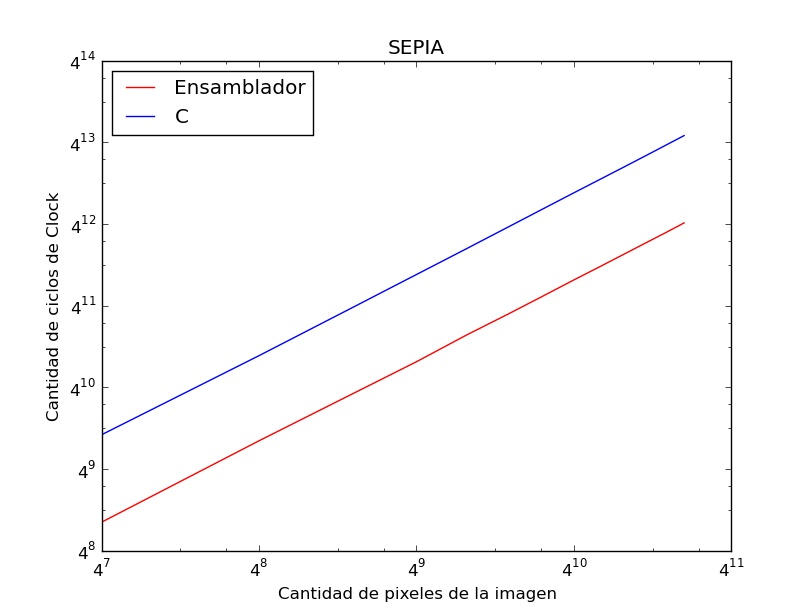
\includegraphics[scale=.4]{./imagenes/sepia-asmVSc.jpeg}
	}
\end{centering}

Observamos en este experimento una brecha no tan amplia como el caso de Cropflip
entre el tiempo que tomó correr los expermientos en C y el que tomó en Assembler, pero resaltando
que los expermientos en assembler requirieron menos ciclos de clock para procesarse.
Esta diferencia era la esperada, debido principalmente a la reducción de accesos a
memoria gracias a la utilización de la tecnología SSE en el código de Assembler. Comparamos también las
mismas implementaciones pero usando diferentes flags de optimización para que
realizara el compilador de C. Los resultados son los que arrojan los siguientes gráficos:

%\begin{figure}[!ht]
%    \centering
%    \begin{floatrow}
%      \ffigbox[\FBwidth]{\caption{Comparación C con flag O3 vs ASM}}{%
%        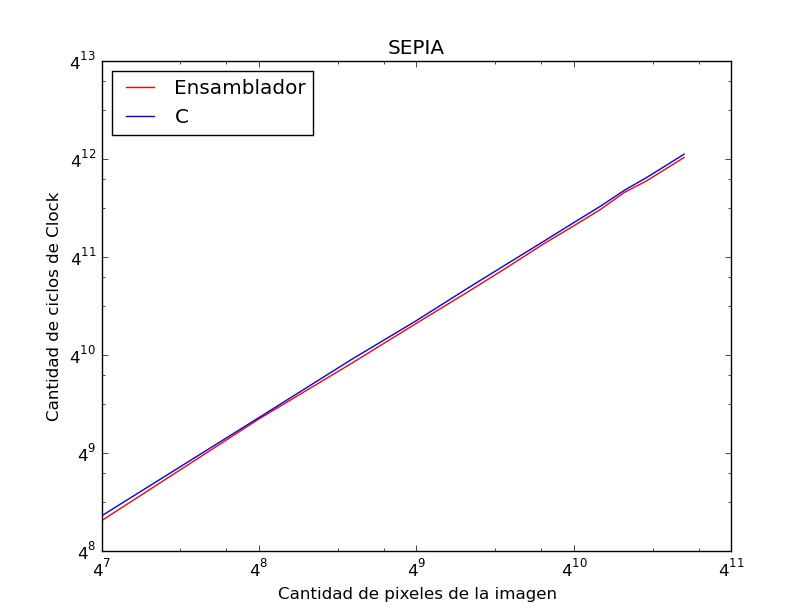
\includegraphics[scale=.25]{./imagenes/sepia-asmVScO3.jpeg}
%      }
%    \end{floatrow}
%\end{figure}

\begin{centering}
\ffigbox[\FBwidth]{\caption{Comparación C con flag O3 vs ASM}}{%
	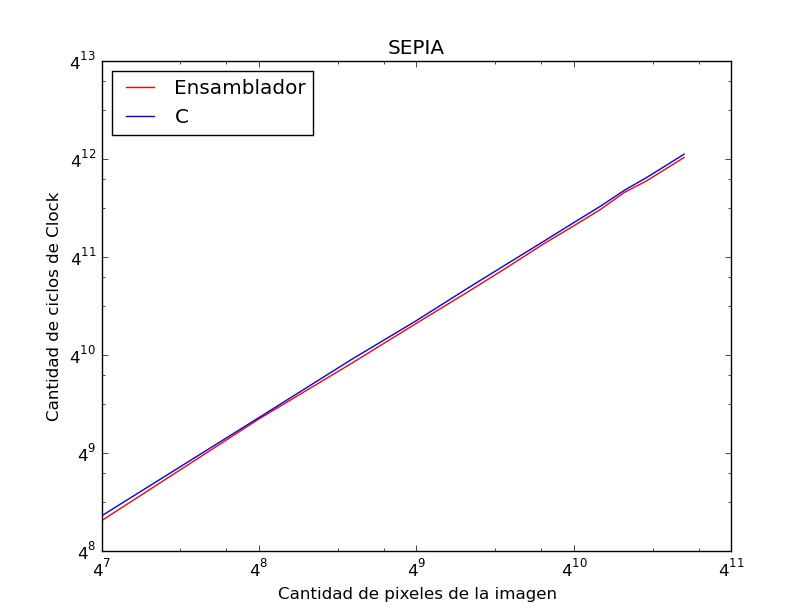
\includegraphics[scale=.4]{./imagenes/sepia-asmVScO3.jpeg}
	}
\end{centering}

Al utilizar el flag de optimización O3, el código generado
por el compilador fue mucho más eficiente. Se observa en el
gráfico una notable disminución de los tiempos de ejecución
del código realizado en C, el cual casi iguala a la performance
del realizado en ASM.

%\begin{figure}[!ht]
%    \centering
%    \begin{floatrow}
%      \ffigbox[\FBwidth]{\caption{Comparación C con flag O3 y mavx vs ASM}}{%
%        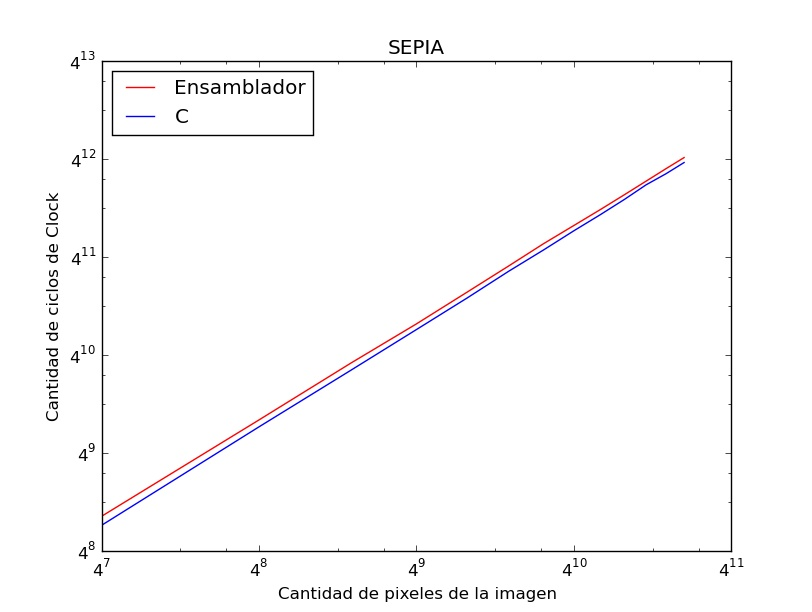
\includegraphics[scale=.25]{./imagenes/sepia-asmVScO3SSE4-2AVX.jpeg}
%      }
%    \end{floatrow}
%\end{figure}

\begin{centering}
\ffigbox[\FBwidth]{\caption{Comparación C con flag O3 y mavx vs ASM}}{%
	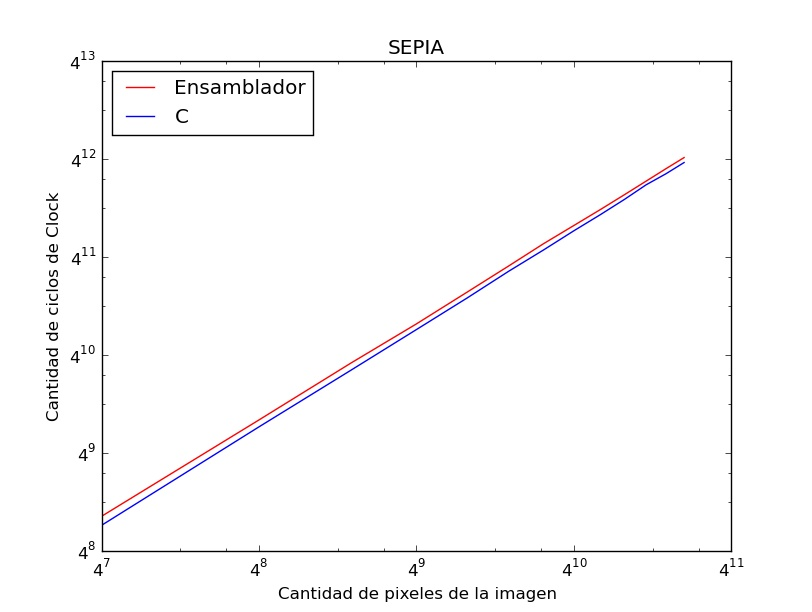
\includegraphics[scale=.4]{./imagenes/sepia-asmVScO3SSE4-2AVX.jpeg}
	}
\end{centering}

Este fue el resultado más interesante. Al compilar con la opción de AVX,
que es una tecnología con nuevas instrucciones y expande los registos de
128 bits a 256 bits, se observa que el código generado por el compilador
de C es ligeramente más óptimo en términos de tiempo de procesamiento que
el realizado por nosotros en assembler. Era un resultado igualmente esperable,
ya que al utilizar registros de 256 bits se reducen aún más los accesos a memoria
necesarios para traer y guardar pixeles. La relación lineal entre tamaño de imagen
y tiempo de procesamiento se mantiene nuevamente en el experimento.

\subsubsection{Low Dynamic Range}
La idea específica de la implementación de este filtro tanto en C como en Assembler es ver pixel por pixel y realizar los cálculos
de sus 25-vecinos por separado. Esto se hace de dos formas distintas dependiendo del lenguaje.
\newline
En el caso de C, primero se realiza la suma de los canales RGB de los 25-vecinos recorriendo pixel por pixel y canal por canal y
eso se va guardando en una misma variable de tamaño int.
Esto hace que por cada pixel y por cada canal, se realice un acceso a memoria. \newline
Una vez obtenido la suma total, se la multiplica por el $\alpha$ pasado por parámetro. y se guarda en una nueva variable de tamaño Float.
Luego, esta nueva variable se la multiplica por separado por cada canal RGB del pixel a modificar y se guarda el resultado tres variables más
de tamaño Float. Después, se realiza la división por "Max", mencionado en la introducción de este informe y se le suma una vez más el canal
correspondiente a modificar del pixel central, guardando otra vez cada resultado en una nueva variable de tamaño Float. Finalmente,
se satura cada variable y se la guarda en cada canal a modificar. Esto se hace una cantidad de veces igual a la cantidad total de pixels
que tiene la imagen salvo por 2 líneas de pixeles en cada borde. Para ese caso, lo único que se hace es copiar los pixeles de la imagen original
a la imagen destino. \newline
Para el caso de Assembler, lo que cambia respecto de la implementación C son la cantidad de accesos a memoria. Esto se corrige utilizando la
tecnología SSE, con los registros de 128-bits, en los cuales al momento de realizar los cálculos de los 25-vecinos se cargan primero los 4 pixels
de cada fila y luego el último pixel de cada una. Además se utilizan instrucciones tales como \textit{phaddw} y \textit{paddw}, las cuales
perimten realizar sumas de datos empaquetados en los registros mencionado. Para el caso de la multiplicación y división, se utilizan las instrucciones
\textit{pmulld} y \textit{divps}, las cuales también trabajan con datos empaquetados en los registros de 128-bits. Para conservar el canal de
transparencia, se utilizan las instrucciones \textit{pextrd}, la cual extrae un Double Word a un registro de 32 bits, y luego \textit{pinsrd},
la cual inserta de un registro de 32 bit un Double Word en un registro de 128 bits. Ambas instrucciones utilizan una máscara que indica cuál
es el Double Word que se desea obtener o modificar.
\newline

En un primer experimento comparamos la implementación en C sin ningún tipo de optimización con la implementación en Assembler. En el gráfico
resultante, se puede observar que ambas implementaciones crecen de manera lineal según el tamaño de la imagen. Sin embargo, la implementación en
Assembler es aún más rápida que la de C.

\noindent%
\begin{minipage}{\linewidth}% to keep image and caption on one page
\makebox[\linewidth]{%        to center the image
  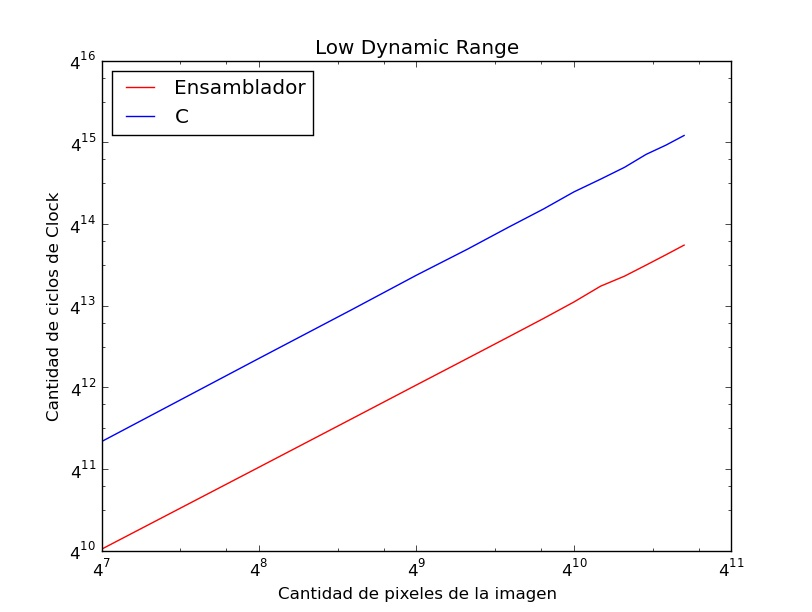
\includegraphics[keepaspectratio=true,scale=0.4]{./imagenes/ldr-asmVSc.jpeg}}
\captionof{figure}{Comparación C sin optimización vs ASM}%\label{visina8}%      only if needed
\end{minipage}
\ \

En el segundo experimento, comparamos la implementación C compilando con el flag de optimización O3. A continuación se puede ver el gráfico del mismo:

\begin{centering}
\ffigbox[\FBwidth]{\caption{Comparación C con optimización O3 vs ASM}}{%
	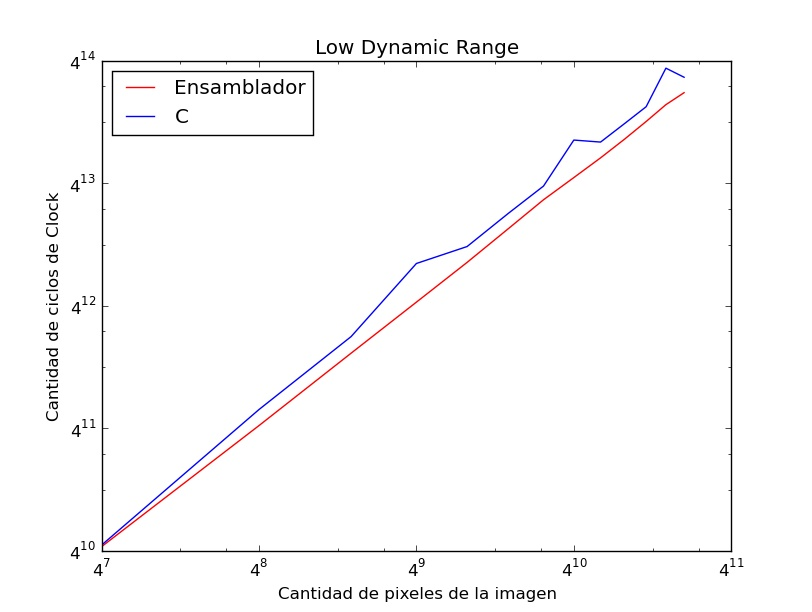
\includegraphics[scale=.4]{./imagenes/ldr-asmVScO3.jpeg}
	}
\end{centering}


Podemos analizar en este caso que el flag O3 realmente cambia el rendimiento de la implementación. Si bien ya no es tán lineal como lo era en el
experimento anterior, ahora se acerca mucho al performance de la implementación en Assembler.
\newline
Como último experimento, agregamos el flag que permite utilizar los registros de 256 bits. Esta vez, se asemeja mucho al experimento anterior, pero
sigue siendo un poco más rápido. El crecimiento de la cantidad de ciclos de procesador que toma, crece respecto del tamaño de la imagen de la misma
forma que sin el flag AVX.

\begin{figure}[!ht]
    \centering
    \begin{floatrow}
      \ffigbox[\FBwidth]{\caption{Comparación C con optimización O3 vs ASM}}{%
        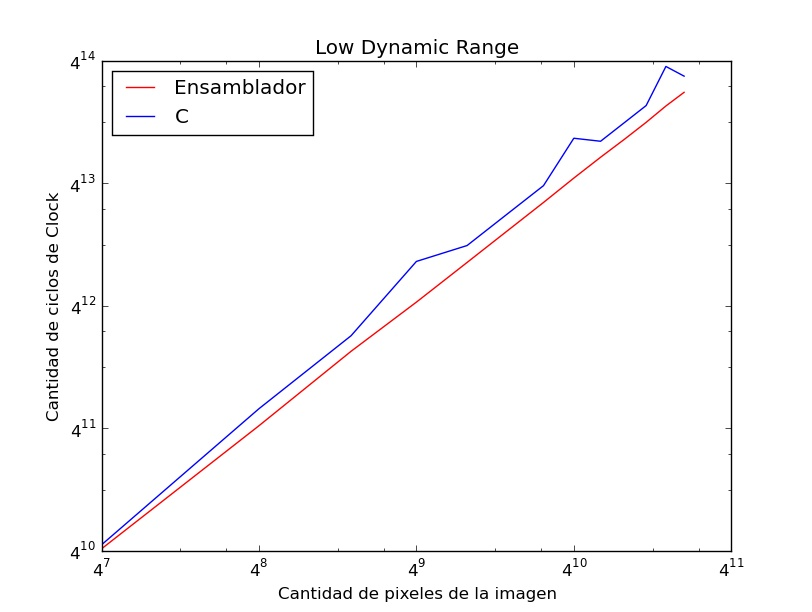
\includegraphics[scale=.4]{./imagenes/ldr-asmVScO3AVX.jpeg}
      }
    \end{floatrow}
\end{figure}

\subsection{Comparación con diferentes implementaciones}
Además de las implementaciones descriptas previamente en este informe, realizamos una segunda implementación en C de Croplfip y otra en ASM de Sepia.
Consideramos que no tendría mucho sentido hacer una segunda implementación en ASM de Cropflip ya que simplemente son copias de memoria a memoria con
pequeños cálculos matemáticos, cosa que se podría hacer en C. En cambio, no hicimos una segunda implementación en C de Sepia ya que la diferencia sí podía hacerse
notoria en ASM, no así en C.

\subsubsection{Cropflip C vs Cropflip C}
La diferencia entre las implementaciones de Croplfip es que en la primera versión, se realizaban algunos cálculos sobre el siguiente pixel a copiar
dentro del mismo loop, lo cual creemos que esto podría afectar en tamaños grandes de imagenes al aplicar el filtro. El siguiente gráfico muestra el tiempo que toma
cada filtro para aplicarse en imágenes que varían en tamaño original pero no en el tamaño que se desea filtrar.

\begin{centering}
\ffigbox[\FBwidth]{\caption{Comparación C  de Cropflip sin optimización}}{%
	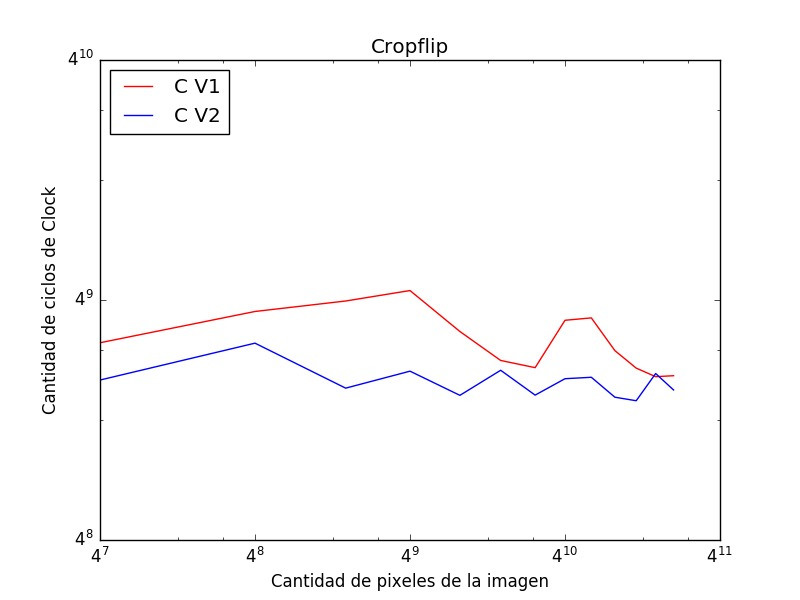
\includegraphics[scale=.55]{./imagenes/implementacionesC-CropflipSinO3.jpeg}
	}
\end{centering}

Podemos notar como la segunda implementación supera a la primera comparando los ciclos de reloj, pero no por mucha diferencia. Tal como esperabamos,
esto ocurre porque son cálculos matemáticos simples, como sumas y restas, y no accesos a memoria o divisiones.
En ambos casos, es un tiempo casi constante más allá del tamaño de la imagen. Al igual que en anteriores experimentos, esto se debe a que el filtro
recorta siempre el mismo tamaño de imagen. Para la primera implementación obtuvimos un tiempo de 171040~ ciclos de reloj en promedio por ejecución, mientras
que para el segundo, el promedio fue de 150064. Casi 20000 ciclos de reloj de diferencia, lo cual es bastante si se tiene en cuenta que la cantidad de
accesos a memoria es la misma en ambos casos.

También comparamos estas dos implementaciones utilizando el flag O3 en el compilador y comparando nuevamente con la verisón de ASM.

\begin{centering}
\ffigbox[\FBwidth]{\caption{Comparación C vs ASM con optimización entre CropflipCv1, CropflipCv2 y CropflipASM}}{%
	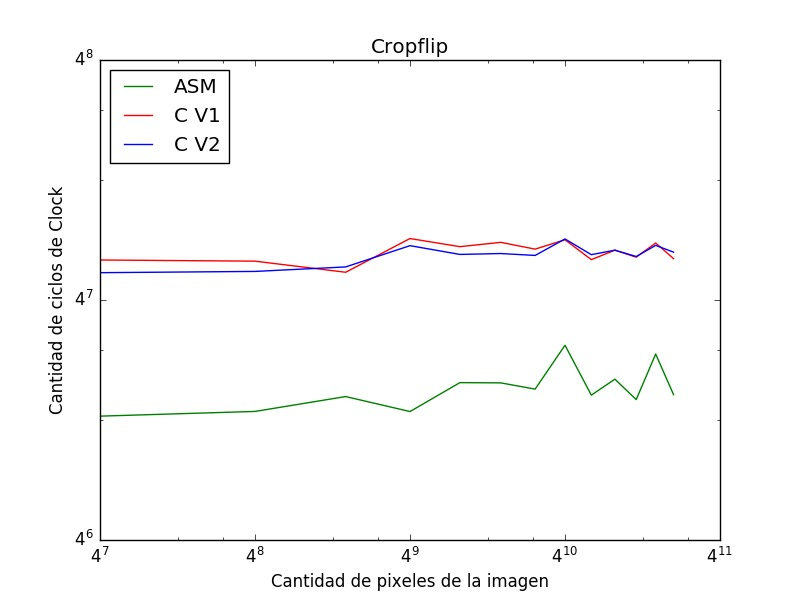
\includegraphics[scale=.55]{./imagenes/implementacionesCASM-cropflipConO3.jpeg}
	}
\end{centering}

En este grafico podemos observar que utilizando el flag de optimización O3, en algunos casos la primera implementación en C de Cropflip puede llegar
a ser levemente superior a la segunda. Esto también implica que la optimizacion que realiza el compilador hace que la diferencia escrita en el código de la segunda versión
 quede prácticamente de lado, ya que evidentemente los ciclos de reloj son casi iguales más allá de si los cálculos de sumas y restas se hacen en el ciclo que recorre la imagen o no.
 Sin embargo, esta comparación no tiene sentido cuando se tiene en cuenta la implementación en ASM, la cual es
ampliamente más rápida que las otras dos. Otra vez vemos que la versión de ASM realiza un mejor trabajo a pesar de ser más dificil de programar.

\subsubsection{Sepia ASM vs Sepia ASM}
En esta segunda implementación el cambio principal fue que en lugar de multiplicar valores de punto flotante para realizar divisiones, se reemplazan
 esos valores por números entereros, multiplicandolos por 10 y luego dividiéndolos por los resultados. La multiplicación por 10 también debió hacerse
en el número con el cual se iba a utilizar como divisores para mantener la relación. Esta vez, esperamos nuevamente que la segunda implementación supere a la primera.

\begin{figure}[!ht]
    \centering
    \begin{floatrow}
      \ffigbox[\FBwidth]{\caption{Comparación ASM}}{%
        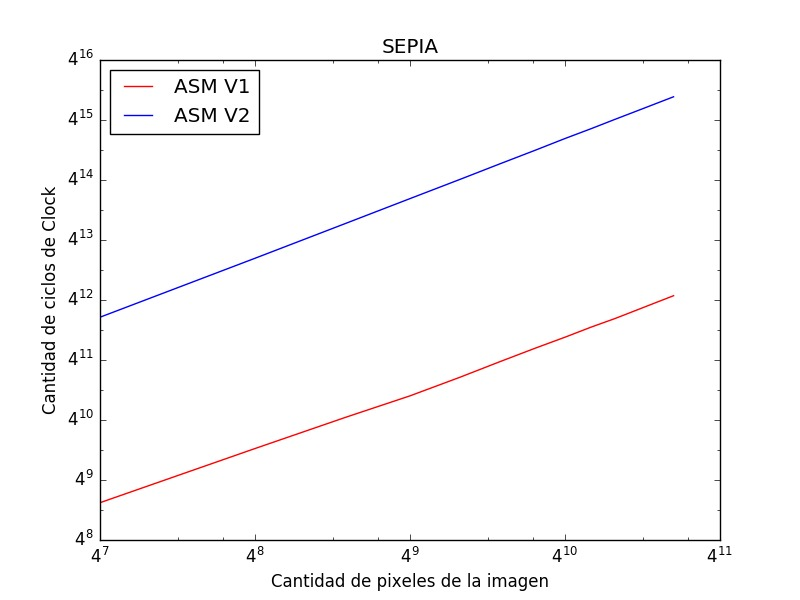
\includegraphics[scale=.55]{./imagenes/implementacionesASM-Sepia.jpeg}
      }
    \end{floatrow}
\end{figure}

Nos llevamos una sopresa al ver que la segunda implementación tomaba notoriamente mucho más tiempo que la primera. Llegamos a la conclusión que esto se debe
a que realizar divisiones es mucho más costoso que multiplicar por unidades de punto flotante.

\subsection{Comparación de imágenes}
Siguiendo con los experimentos, realizamos una serie de ejecuciones del filtro LDR con imágenes de distintos colores. Siempre utilizando imágenes de
tamaño 512x512px y aplicando el filtro 100000 veces por imagen con un alpha de 250. Utilizamos en este experimento una imagen completamente roja, una verde, una azul (es decir,
una por cada color base de RGB, colocando cada pixel en el máximo de ese canal y los otros en 0), una blanca (todos los canales RGB en 255), una negra
(los canales RGB en 0) y por último una imágen con colores variados.

\subsubsection{Análisis de tiempos de clock entre todas las imágenes}
Nuestra hipótesis era que al ser un filtro en el que solo se realizan cuentas matemáticas
más allá del color de cada pixel y no se hacen, por ejemplo, accesos a memoria si un pixel tiene tal color o que si por la suma de otros se hace tal cosa. Entonces,
pusimos a prueba esta idea y plasmamos en un gráfico de barras los datos obtenidos de calcular el promedio de la cantidad de ciclos de reloj por cada ejecucion del filtro
en cada imagen.

\begin{figure}[!ht]
    \centering
    \begin{floatrow}
      \ffigbox[\FBwidth]{\caption{Comparación entre imágenes de distintos colores}}{%
        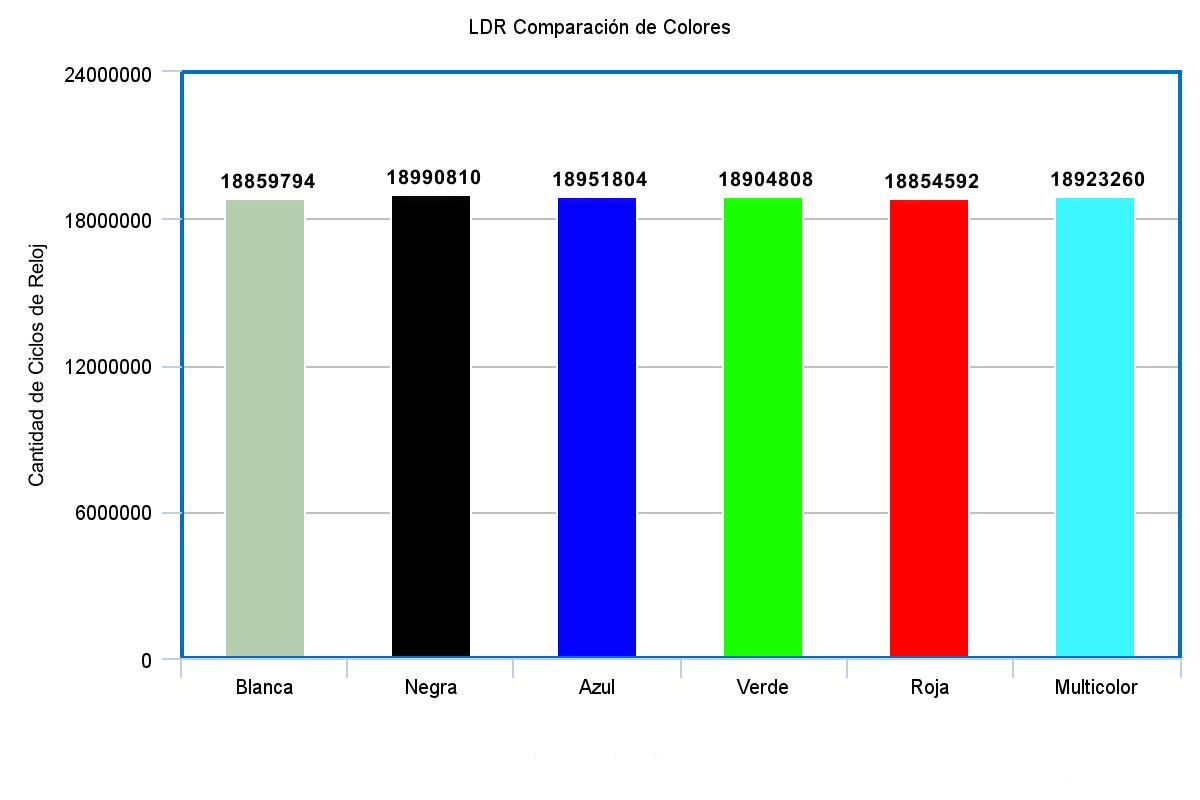
\includegraphics[scale=.3]{./imagenes/meta-chart.jpeg}
      }
    \end{floatrow}
\end{figure}

Observamos en este gráfico que, efectivamente, hubo diferencias en la cantidad de ciclos de reloj promedio por ejecución dependiendo de los colores de la imagen,
sin embargo, esta diferencia no es tan notoria como sí puede ser la diferencia de aplicar el filtro implementado en C o en Assembler.
Para dar datos más precisos, la mayor diferencia entre las imágenes probadas es entre la imagen negra y la roja. Tomando la diferencia en ciclos de reloj
parece ser bastante, pero en porcentaje, la demora que tiene el filtro en la imagen negra respecto de la roja es de menos de un 1\%.
Incluso en ciclos de reloj, se puede notar la cercanía al volver al experimento de C vs ASM, en el que se pueden llegar a observar diferencias de, por ejemplo,
115139916 ciclos de reloj (C vs ASM del filtro LDR en una imagen de 512x512).

\subsubsection{Análisis por imágen}
Lo último que realizamos en cuanto al análisis de imagenes de colores lisos fue ver cómo cambiaban según el $\alpha$ que se pasa por parámetro
para LDR. Nuestra hipótesis esta vez fue que cambiaría todas lás imagenes cuando se le pase un $\alpha$ negrativo excepto a la imagen negra, la cual
no cambiaría en absoluto para ningún $\alpha$.

En el anexo de comparación de imágenes lisas se pueden ver las imagenes originales y sus versiones en ldr con $\alpha$ $255$ y $-255$.

Lo que pudimos notar al ver las imagenes que obtuvimos fue que todas (excepto la negra y la blanca que son un caso separado) varían más
cuando se utilizaba el $\alpha$ negativo pero que de todas formas se percibía una diferencia con las que se usaba el $\alpha$ positivo.

Para el caso de la imagen blanca, fue sorprendente ver cómo se transformó básicamente en una imagen completamente negra cuando se utilizó el $\alpha$
negativo, mientras que para el positivo era, como se esperaba, la misma imagen. Eso se debe a que en el formato RGB, el color blanco se representa por
[255, 255, 255], por lo que al utilizar el $\alpha$ positivo, la imagen simplemente satura a 255 cada canal; al usar el $\alpha$ negativo, es básicamente
hacer que cada canal de cada pixel sature a 0.
Por último, para la imagen negra fue exactamente lo esperado. Al representarse en el formato RGB como [0, 0, 0], multiplicar cualquier valor en cualquier canal
haría simplemente que siga siendo 0, y eso es parte del funcionamiento del filtro ldr, sumas y multiplicaciones, pero que en este caso darían siempre 0.

\subsection{Comparación entre Compiladores}
Un compilador no es mas que un programa que basicamente toma el codigo C
y lo traduce a codigo de maquina. Existen varios para C, tales como como GCC (el cual se usa en gran parte de este trabajo), Clang y el Compilador de Intel.
Lo que hicimos en este experimento fue compilar los filtros con GCC y Clang en sus versiones 5.3.1 y 3.8.0 respectivamente, para luego realizar la comparación.
%Lo que vamos a hacer es compilar el codigo con Clang/GCC y ver si encontramos diferencias.Para comparar, se van a usar la version 4.8.4 de GCC y la 3.4 de Clang.
%Para realizar la comparacion, vamos a compilar el TP con GCC y luego con Clang.
%Para empezar, vamos a comparar con optimizacion nula
Nuestra hipótesis para este experimento es que el compilador de GCC optimiza más el código producido que Clang, ya que en caso contrario, este último estaría instalado por defecto
en muchos de los sistemas operativos existentes en lugar de GCC (teniendo en cuenta las muchas otras razones por las que puede no ser el caso).


Aqui el grafico de GCC sin optimización

\begin{figure}[H]
    \centering
    \begin{floatrow}
      \ffigbox[\FBwidth]{\caption{Filtros con GCC -O0}}{%
        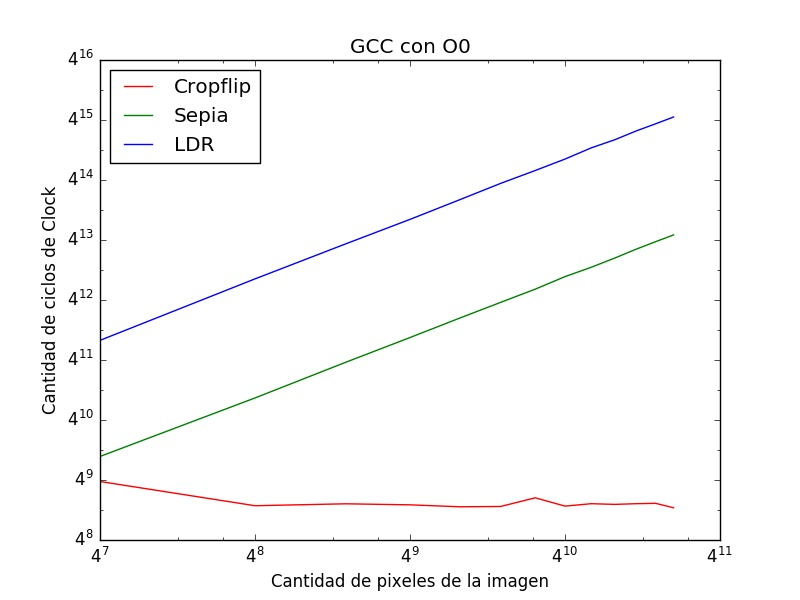
\includegraphics[scale=.55]{./imagenes/GCC0.jpg}
      }
    \end{floatrow}
\end{figure}


Aca vemos que Cropflip, que es el filtro más rápido, empieza tomando $4^9$ ciclos de reloj en la imagen más chica y finaliza cerca de la mitad entre $4^8$ y $4^9$.
Los otros dos filtros alcanzan hasta $4^{13}$ y $4^{15}$ ciclos de reloj.

Aqui el grafico de Clang

\begin{figure}[H]
    \centering
    \begin{floatrow}
      \ffigbox[\FBwidth]{\caption{Filtros con Clang -O0}}{%
        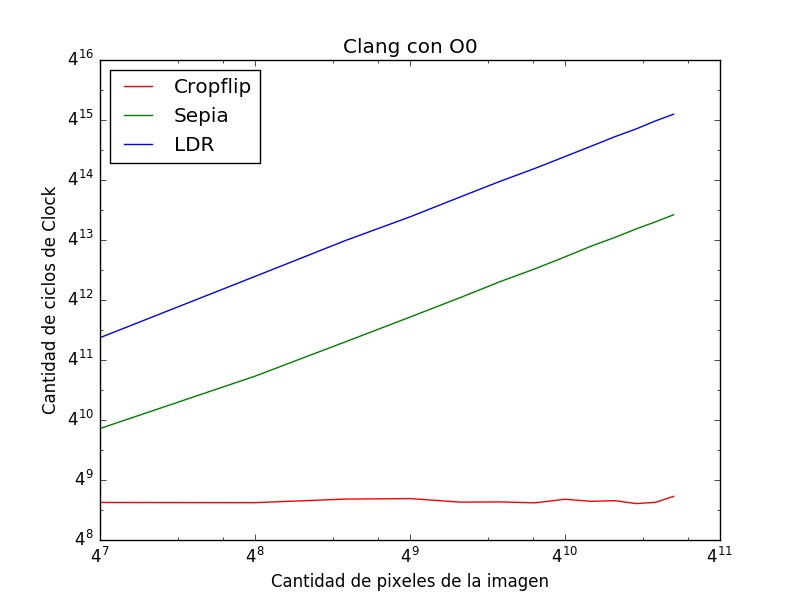
\includegraphics[scale=.55]{./imagenes/Clang0.jpg}
      }
    \end{floatrow}
\end{figure}

Tras este gráfico, observamos que las diferencias de LDR y Sepia son casi nulas entre los compiladores, sin embargo Cropflip tiene la diferencia de que es más
constante en cuanto a ciclos de reloj sobre tamaño de la imagen.


Ahora, vamos a repetir el mismo experimento pero variando las flags, esta vez vamos a usar 03. Como hipotesis, esperamos ver un comportamiento similar al visto en O0.
\begin{figure}[H]
    \centering
    \begin{floatrow}
      \ffigbox[\FBwidth]{\caption{Filtros con GCC -O3}}{%
        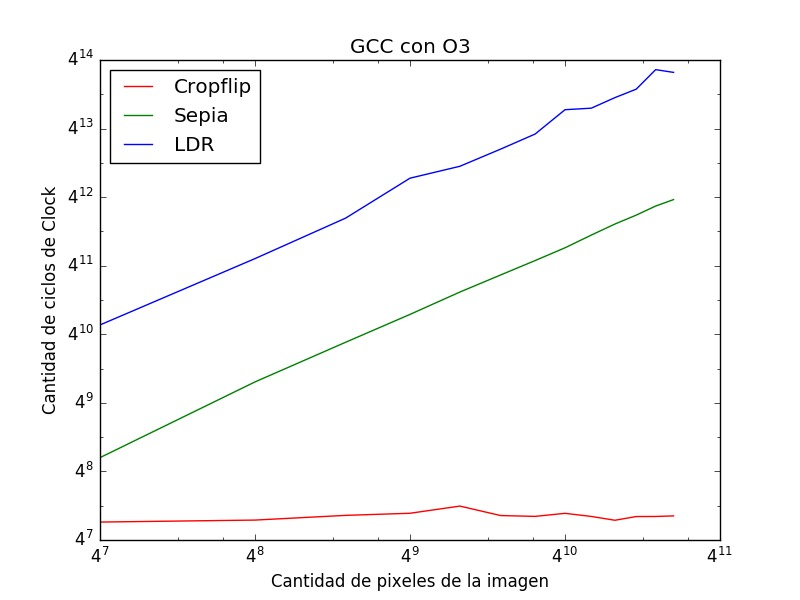
\includegraphics[scale=.55]{./imagenes/GCC3.jpg}
      }
    \end{floatrow}
\end{figure}


\begin{figure}[H]
    \centering
    \begin{floatrow}
      \ffigbox[\FBwidth]{\caption{Filtros con Clang -O3}}{%
        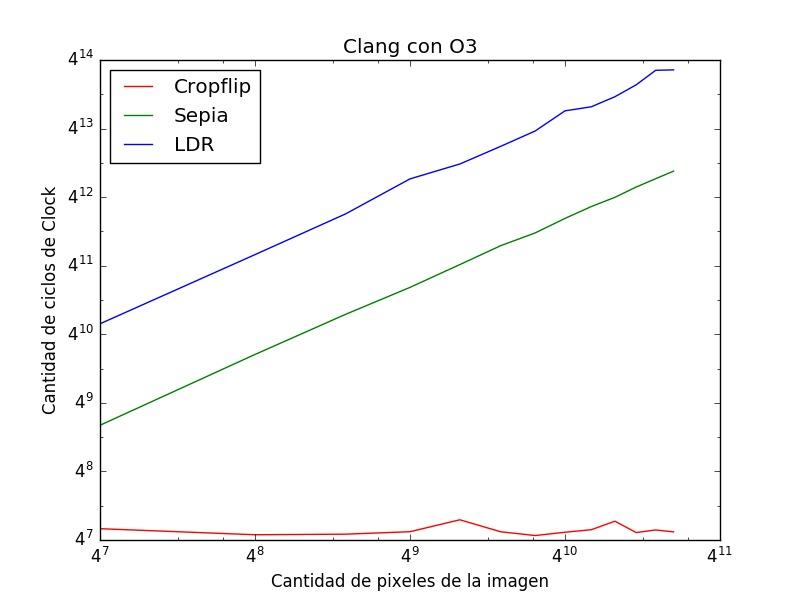
\includegraphics[scale=.55]{./imagenes/Clang3.jpg}
      }
    \end{floatrow}
\end{figure}

Ciertamente, se observó lo esperado. Tienen un comportamiento muy similar más allá de los flags de optimización. Podemos entender entonces que la desición
sobre usar un compilador u otro quedaría simplemente por preferencia y no por performance.


\section{Conclusiones y trabajo futuro}

Como conclusiones generales podemos destacar que los algoritmos implementados
en código Assembler con el uso de instrucciones SSE de Intel son más óptimos que
las implementaciones de los algoritmos en C (que se compilaron sin ningún
tipo de optimización). Esto se debe principalmente a
su capacidad de procesar múltiples datos al mismo tiempo, generando un efecto
de paralelismo en el procesamiento y reduciendo la cantidad de accesos a memoria.
No obstante, al utilizar flags de optimización en la compilación de los algoritmos
implementados en C, la situación cambió en algunos expermientos. Para el caso particular
del filtro sepia, resultó ligeramente más óptima en términos de tiempo de ejecución
la implementación en C, compilada con optimización O3 y para que utilize la tecnología
AVX con registros de 256 bits, que la implementación realizada en Assembler. Esto puede deberse
a que al tener registros aún más grandes que los utilizados en Assembler (SSE de 128 bits),
el código que generó el compilador permite procesar aún más datos en paralelo.
Para el caso de Low Dynamic Range se notó una mejoría significativa usando la misma optimización
pero que no alcanzó a igualar o superar al código realizado en Assembler. En el caso de Cropflip, la mejoría no fue significativa.
Por último, es importante destacar que el tiempo necesario para implementar un filtro en lenguaje
Assembler es superior al del necesario para realizarlo en un lenguage de un nivel de abstración
un poco más alto como es C. Si bien se observan diferencias significativas en la mayoría de los
casos en cuestiones de performance, también conviene tener en cuenta el costo de implementación y
analizar en cada caso y contexto de uso si el esfuerzo y tiempo adicional justifican los resultados,
ya que como se mencionó antes, se puede obtener un muy buen resultado sólo usando optimizaciones del compilador en C.

\par
Como siguientes pasos a realizar para este trabajo se pueden realizar
muchas más implementaciones de los filtros en el lenguaje Assembler para comparar
su performance. Por ejemplo, para el caso de LDR, se podría realizar una implementación
que además de trabajar con los 25 vecinos de un pixel con registros de 128 bits paralelamente,
también se almacenen en registros de 128 bits las sumas parciales de estos 25 vecinos para que
no haya que calcularlas todas nuevamente para el pixel próximo. La idea sería que solamente se
tenga que computar lo que cambia, y lo que de alguna manera permanezca igual se puede almacenar.
Esto reduciría los accesos a memoria y las operaciones a realizar, lo que supondría una mejora en
el tiempo de ejecución que llevaría el filtro. Para el caso de
Cropflip no hay muchas formas de realizar la copia a memoria de la nueva imagen. Se podría probar
con una implementación que recorra la imagen en otro orden o que la copie a memoria en otro orden,
pero esto no supondría una diferencia significativa. Se podría usar instrucciones de la tecnología
de AVX de Intel en caso de que el procesador lo admita, tanto para este último filtro como para todos.
En el caso de usar la tecnología de AVX, todos las implementaciones deberían tener un tiempo de
procesamiento menor que las anteriores, ya que con registros de 256 bits y nuevas instrucciones se pueden
procesar aún más datos paralelamente.

\newpage
\section{Anexo de comparación de imágenes lisas}


 \begin{figure}[!ht]
     \centering
     \begin{floatrow}
       \ffigbox[\FBwidth]{\caption{Blanca original}}{%
         
\includegraphics[scale=.2]{./imagenes/blanca.jpg}
       }
			 \ffigbox[\FBwidth]{\caption{Blanca con $\alpha$ $255$}}{%
         
\includegraphics[scale=.2]{./imagenes/blanca-255.jpeg}
       }
			 \ffigbox[\FBwidth]{\caption{Blanca con $\alpha$ $-255$}}{%
         
\includegraphics[scale=.2]{./imagenes/blanca--255.jpeg}
       }
     \end{floatrow}
 \end{figure}

 \begin{figure}[!ht]
     \centering
     \begin{floatrow}
       \ffigbox[\FBwidth]{\caption{Negra original}}{%
         
\includegraphics[scale=.2]{./imagenes/negra.jpg}
       }
			 \ffigbox[\FBwidth]{\caption{Negra con $\alpha$ $255$}}{%
         
\includegraphics[scale=.2]{./imagenes/negra-255.jpeg}
       }
			 \ffigbox[\FBwidth]{\caption{Negra con $\alpha$ $-255$}}{%
         
\includegraphics[scale=.2]{./imagenes/negra--255.jpeg}
       }
     \end{floatrow}
 \end{figure}

 \begin{figure}[!ht]
     \centering
     \begin{floatrow}
       \ffigbox[\FBwidth]{\caption{Roja original}}{%
         
\includegraphics[scale=.2]{./imagenes/roja.jpg}
       }
			 \ffigbox[\FBwidth]{\caption{Blanca con $\alpha$ $255$}}{%
         
\includegraphics[scale=.2]{./imagenes/roja-255.jpeg}
       }
			 \ffigbox[\FBwidth]{\caption{Blanca con $\alpha$ $-255$}}{%
         
\includegraphics[scale=.2]{./imagenes/roja--255.jpeg}
       }
     \end{floatrow}
 \end{figure}

 \begin{figure}[!ht]
     \centering
     \begin{floatrow}
       \ffigbox[\FBwidth]{\caption{Azul original}}{%
         
\includegraphics[scale=.2]{./imagenes/azul.jpg}
       }
			 \ffigbox[\FBwidth]{\caption{Azul con $\alpha$ $255$}}{%
         
\includegraphics[scale=.2]{./imagenes/azul-255.jpeg}
       }
			 \ffigbox[\FBwidth]{\caption{Azul con $\alpha$ $-255$}}{%
         
\includegraphics[scale=.2]{./imagenes/azul--255.jpeg}
       }
     \end{floatrow}
 \end{figure}

 \begin{figure}[!ht]
     \centering
     \begin{floatrow}
       \ffigbox[\FBwidth]{\caption{Verde original}}{%
         
\includegraphics[scale=.2]{./imagenes/verde.jpg}
       }
			 \ffigbox[\FBwidth]{\caption{Verde con $\alpha$ $255$}}{%
         
\includegraphics[scale=.2]{./imagenes/verde-255.jpeg}
       }
			 \ffigbox[\FBwidth]{\caption{Verde con $\alpha$ $-255$}}{%
         
\includegraphics[scale=.2]{./imagenes/verde--255.jpeg}
       }
     \end{floatrow}
 \end{figure}

 \begin{figure}[!ht]
     \centering
     \begin{floatrow}
       \ffigbox[\FBwidth]{\caption{Colores original}}{%
         
\includegraphics[scale=.27]{./imagenes/colores.jpeg}
       }
			 \ffigbox[\FBwidth]{\caption{Blanca con $\alpha$ $255$}}{%
         
\includegraphics[scale=.27]{./imagenes/colores-255.jpeg}
       }
			 \ffigbox[\FBwidth]{\caption{Blanca con $\alpha$ $-255$}}{%
         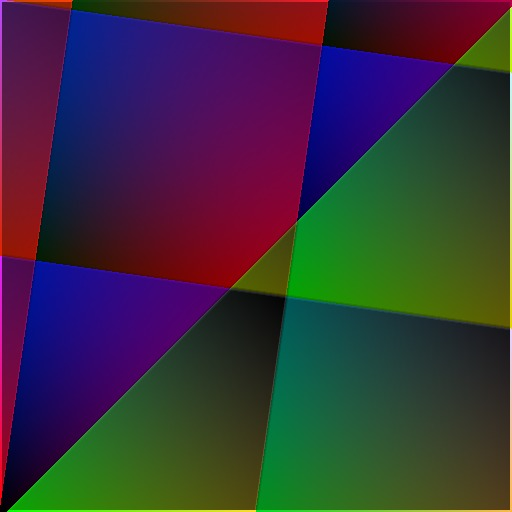
\includegraphics[scale=.27]{./imagenes/colores--255.jpeg}
       }
     \end{floatrow}
 \end{figure}

%\begin{codesnippet}
%\begin{verbatim}

%struct Pepe {

 %   ...

%};

%\end{verbatim}
%\end{codesnippet}

\end{document}
